\documentclass{article}[11pt]

\usepackage{amsmath}
\usepackage{amssymb}
\usepackage{nicefrac}

\usepackage{pdflscape}

\usepackage{upgreek}

\usepackage{bashful}

% No intendation
\setlength\parindent{0pt}

\usepackage{hyperref}

\usepackage{siunitx}
\sisetup{
  per-mode=fraction,
  fraction-function=\tfrac
}

\usepackage{listings}
  \lstset{
    basicstyle=\ttfamily,
    escapeinside=||,
    xleftmargin=1cm
  }

\usepackage{float}

\usepackage{longtable}

\usepackage{multirow}

\usepackage{tikz}
  \usetikzlibrary{patterns}
  \usetikzlibrary{arrows.meta}
  \usetikzlibrary{shapes.misc}
  \usetikzlibrary{calc}

\usepackage{pgfplots}

\usepackage{cleveref}
\crefmultiformat{equation}{(#2#1#3)}{ and~(#2#1#3)}{, (#2#1#3)}{ and~(#2#1#3)}


\usepackage{acronym}
\usepackage[acronym,nonumberlist]{glossaries}
\glsdisablehyper
\makeglossaries
\newacronym{spice}{SPICE}{Simulation Program with Integrated Circuit Emphasis}
\newacronym{lef}{LEF}{Library Exchange Format}
\newacronym{dft}{DFT}{Discrete Fourier Transform}
\newacronym{dtft}{DTFT}{Discrete-Time Fourier Transform}
\newacronym{fft}{FFT}{Fast Fourier Transform}
\newacronym{mosfet}{MOSFET}{Metal–Oxide–Semiconductor Field-Effect Transistor}
\newacronym{clm}{CLM}{Channel Length Modulation}
\newacronym{de}{DE}{differential equation}
\newacronym{soi}{SOI}{silicon-on-insulator}
\newacronym{ldo}{LDO}{low-dropout regulator}
\newacronym{ota}{OTA}{operational-transconductance amplifier}
\newacronym{ofa}{OFA}{operational-floating amplifier}

% literature
\usepackage[ backend=biber
           , isbn=true
           , sorting=none
           , style=ieee
           ]{biblatex}
\addbibresource{./../../literature.bib}

% definitions
\def \whatis       {Notes}
\def \title        {Fuubar}

\def \author       {Matthias Schweikardt}

\def \authorMail   {mschweikardt@posteo.de}

\def \authorGithub {mschweikardt}

\def \license      {CC BY-SA 4.0}
\def \licenseUrl   {https://creativecommons.org/licenses/by-sa/4.0/}

\def \date         {nodate}

\def \pdfurl       {https://mschweikardt.github.io/ee-notes/%
\bash[stdout]
IFS=/ 
var=($PWD)
echo ${var[-1]}
\END%
.pdf
}
\def \srcurl       {srcurl}


% Customize footer and header of document
\usepackage{fancyhdr}

% Access last page number
\usepackage{lastpage}

% Access last page number
\usepackage[thinc]{esdiff}

% Physics
\usepackage{physics}

% Comment environment
\usepackage{comment}

% Subcaptions
\usepackage{subcaption}

% Thicker lines in tables
\usepackage{booktabs}

% Indentation in footnote
\makeatletter
\renewcommand\@makefntext[1]{\leftskip=2em\hskip-0.5em\@makefnmark#1}
\makeatother         

% qty with the siunitx definition
\AtBeginDocument{\RenewCommandCopy\qty\SI}

% TikZ compatibility
\pgfplotsset{compat=1.18}


\makeatletter
\pgfmathdeclarefunction{myatan2}{2}{%
\begingroup%
  \pgfmathfloattofixed{#1}\edef\tempa{\pgfmathresult}%
  \pgfmathfloattofixed{#2}%
  \pgfkeys{pgf/fpu=false}%
  \pgfmathparse{atan2(\tempa,\pgfmathresult)}\pgfkeys{/pgf/fpu}%
  \pgfmathfloatparsenumber{\pgfmathresult}%
  \pgfmath@smuggleone\pgfmathresult%
\endgroup
}
\makeatother

\usepackage{tabularx}
% usepackages
\usepackage[ a4paper
           , textwidth  = 16.0cm
           , textheight = 25.0cm
           , headsep    =  0.25cm
           , voffset    =  0.3cm
           , footskip   =  1.25cm
           ]{geometry}

% Section and subsection enumeration
\renewcommand{\thesection}{\Roman{section}.} 
\renewcommand{\thesubsection}{\thesection\Alph{subsection}}

\usepackage{titlesec}
\titleformat{\section}
  {\normalfont\Large\bfseries}{\thesection}{0.2em}{}
\titleformat{\subsection}
  {\normalfont\large\bfseries}{\thesubsection}{0.2em}{}


% Defince title of document
\newcommand{\notetitle}{
  \begingroup
  \hypersetup{hidelinks}
  \thispagestyle{notefirst}
  \begin{center}
  \rule{\textwidth}{1pt}\\
  \medskip
  {\it \whatis}\\
  \bigskip
  {\LARGE \textbf{\title}}\\
  \medskip
  {\small \author}\\
  \rule{\textwidth}{0.5pt}\\
  {\small
    \begin{minipage}[t]{0.5\textwidth}
      \begin{tabular}[t]{ p{2.25cm} p{5.75cm}}
        Mail: & \href{mailto:\authorMail}{\tt{\authorMail}} \\
        Github: & \href{https://github.com/\authorGithub}{\tt{\authorGithub}} \\
      \end{tabular}
    \end{minipage}%
    %
    \begin{minipage}[t]{0.5\textwidth}
      \begin{tabular}[t]{ p{2.25cm} p{5.75cm} }
        Date: & \date  \\
        License: & \href{\licenseUrl}{\license}
      \end{tabular}
    \end{minipage}
  }%
  {\small
    \begin{minipage}[t]{\textwidth}
      \begin{tabular}[t]{ p{2.25cm} p{12cm}}
        Latest PDF: & \href{\pdfurl}{\tt{\pdfurl}} \\
        Latest Source: & \href{\srcurl}{\tt{\srcurl}}
      \end{tabular}
    \end{minipage}%
  }
  \bigskip
  \rule{\textwidth}{1pt}
  \end{center}
  \endgroup
}

% Header and footer on first page
\fancypagestyle{notefirst}{
  \fancyhf{}
  \renewcommand{\headrulewidth}{0pt}
  \renewcommand{\footrulewidth}{0pt}

  \fancyfoot[C]{\thepage/\pageref*{LastPage}}
}

% Header and footer on 2nd-last page
\fancypagestyle{noterest}{
  \fancyhf{}
  \renewcommand{\headrulewidth}{0.5pt}
  \renewcommand{\footrulewidth}{0.0pt}

  \fancyhead[L]{\author}
  \fancyhead[C]{\title}
  \fancyhead[R]{\date}

  \fancyfoot[C]{\thepage/\pageref*{LastPage}}
}
\pagestyle{noterest}

\usepackage{amsmath}
\usepackage{amssymb}
\usepackage{nicefrac}

\usepackage{pdflscape}

\usepackage{upgreek}

\usepackage{bashful}

% No intendation
\setlength\parindent{0pt}

\usepackage{hyperref}

\usepackage{siunitx}
\sisetup{
  per-mode=fraction,
  fraction-function=\tfrac
}

\usepackage{listings}
  \lstset{
    basicstyle=\ttfamily,
    escapeinside=||,
    xleftmargin=1cm
  }

\usepackage{float}

\usepackage{longtable}

\usepackage{multirow}

\usepackage{tikz}
  \usetikzlibrary{patterns}
  \usetikzlibrary{arrows.meta}
  \usetikzlibrary{shapes.misc}
  \usetikzlibrary{calc}

\usepackage{pgfplots}

\usepackage{cleveref}
\crefmultiformat{equation}{(#2#1#3)}{ and~(#2#1#3)}{, (#2#1#3)}{ and~(#2#1#3)}


\usepackage{acronym}
\usepackage[acronym,nonumberlist]{glossaries}
\glsdisablehyper
\makeglossaries
\newacronym{spice}{SPICE}{Simulation Program with Integrated Circuit Emphasis}
\newacronym{lef}{LEF}{Library Exchange Format}
\newacronym{dft}{DFT}{Discrete Fourier Transform}
\newacronym{dtft}{DTFT}{Discrete-Time Fourier Transform}
\newacronym{fft}{FFT}{Fast Fourier Transform}
\newacronym{mosfet}{MOSFET}{Metal–Oxide–Semiconductor Field-Effect Transistor}
\newacronym{clm}{CLM}{Channel Length Modulation}
\newacronym{de}{DE}{differential equation}
\newacronym{soi}{SOI}{silicon-on-insulator}
\newacronym{ldo}{LDO}{low-dropout regulator}
\newacronym{ota}{OTA}{operational-transconductance amplifier}
\newacronym{ofa}{OFA}{operational-floating amplifier}

% literature
\usepackage[ backend=biber
           , isbn=true
           , sorting=none
           , style=ieee
           ]{biblatex}
\addbibresource{./../../literature.bib}

% definitions
\def \whatis       {Notes}
\def \title        {Fuubar}

\def \author       {Matthias Schweikardt}

\def \authorMail   {mschweikardt@posteo.de}

\def \authorGithub {mschweikardt}

\def \license      {CC BY-SA 4.0}
\def \licenseUrl   {https://creativecommons.org/licenses/by-sa/4.0/}

\def \date         {nodate}

\def \pdfurl       {https://mschweikardt.github.io/ee-notes/%
\bash[stdout]
IFS=/ 
var=($PWD)
echo ${var[-1]}
\END%
.pdf
}
\def \srcurl       {srcurl}


% Customize footer and header of document
\usepackage{fancyhdr}

% Access last page number
\usepackage{lastpage}

% Access last page number
\usepackage[thinc]{esdiff}

% Physics
\usepackage{physics}

% Comment environment
\usepackage{comment}

% Subcaptions
\usepackage{subcaption}

% Thicker lines in tables
\usepackage{booktabs}

% Indentation in footnote
\makeatletter
\renewcommand\@makefntext[1]{\leftskip=2em\hskip-0.5em\@makefnmark#1}
\makeatother         

% qty with the siunitx definition
\AtBeginDocument{\RenewCommandCopy\qty\SI}

% TikZ compatibility
\pgfplotsset{compat=1.18}


\makeatletter
\pgfmathdeclarefunction{myatan2}{2}{%
\begingroup%
  \pgfmathfloattofixed{#1}\edef\tempa{\pgfmathresult}%
  \pgfmathfloattofixed{#2}%
  \pgfkeys{pgf/fpu=false}%
  \pgfmathparse{atan2(\tempa,\pgfmathresult)}\pgfkeys{/pgf/fpu}%
  \pgfmathfloatparsenumber{\pgfmathresult}%
  \pgfmath@smuggleone\pgfmathresult%
\endgroup
}
\makeatother

\usepackage{tabularx}

\def \title  {Duelling Current Sources}
\def \date   {February 25, 2026}

\def \pdfurl {https://mschweikardt.github.io/ee-notes/duelling-current.pdf}
\def \srcurl {https://github.com/mschweikardt/ee-notes/tree/main/notes/duelling-current}

\usepackage[scale=5]{draftwatermark}

\begin{document}

\notetitle

\begin{figure}[H]
  \centering
  \begin{circuitikz}
    \coordinate (out) at (0,0);

    \draw (out) to [short,-] ++ (0,-0.5) 
                to [short,-,i_=$I_{\mathrm{D,N}}$] ++ (0,-0.1) 
                node[nmos, anchor=drain] (nmos) {MN};

    \draw (out) to [short,-] ++ (0,0.5) 
                to [short,-,i<=$I_{\mathrm{D,P}}$] ++ (0,0.1) 
                node[pmos, anchor=drain] (pmos) {MP};

    \draw (nmos.gate) to [short,-] ++ (-1,0)
                      to [V,v=$V_{\mathrm{GS,N}}$] ++ (0,-1.5) coordinate (x)
                      to [short,-*] (x-|nmos.source) coordinate (gnd)
                      to [short,-]  (nmos.source);

    \draw (pmos.gate) to [short,-] ++ (-1,0)
                      to [V,v_=$V_{\mathrm{GS,P}}$] ++ (0,1.5) coordinate (x)
                      to [short,-*] (x-|pmos.source) coordinate (x)
                      to [short,-]  (pmos.source);

    \node[vdd] at (x) {};
    \node[vss] at (gnd) {}; 

    \draw (gnd) to [short,-o] ++ (1.5,0) coordinate (outn);
    \draw (out) to [short,*-o] (out-|outn) coordinate (outp);   

    \path [voltarrow] (outp) edge[] 
      node[midway,below right,inner sep=1pt] 
      {$V_{\mathrm{O}}$} (outn);     
  \end{circuitikz}
  \caption{Duelling Current Sources}
  \label{fig:duell-current}
\end{figure}

\begin{figure}[H]
  \centering
  \begin{subfigure}[b]{0.31\textwidth}
    \centering
    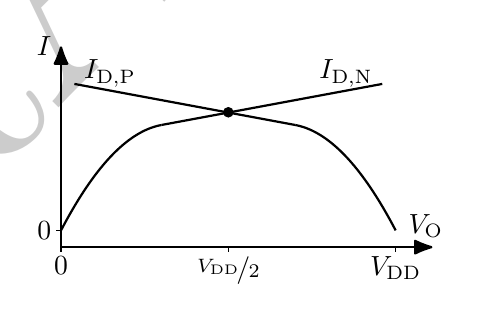
\begin{tikzpicture}[scale=0.85]
      \node[anchor=north] at (0,0) {0};
      \draw[thin] (0,0) -- (0,-0.075);
      \node[anchor=east] at (0,0.25) {0};
      \draw[thin] (0,0.25) -- (-0.075,0.25);

      \node[anchor=north] at (2.5,0) {$\nicefrac{V_{\mathrm{DD}}}{2}$};
      \draw[thin] (2.5,0) -- (2.5,-0.075);
      \node[anchor=north] at (5.0,0) {$V_{\mathrm{DD}}$};
      \draw[thin] (5.0,0) -- (5.0,-0.075);

      \draw[{Latex[round,scale=1.2]}-{Latex[round,scale=1.2]},thick] 
        (0,3) -- (0,0) -- (5.55,0);

      \node[anchor=south] at (5.45,0) {$V_{\mathrm{O}}$};
      \node[anchor=east] at (0,3) {$I$};

      \draw[thick] plot[smooth,domain=0:1.5] (\x, {0.25-0.576033058*\x^2+1.914049588*\x});
      \draw[thick] plot[smooth,domain=1.5:4.8] (\x, {0.185950413*(\x-1.5)+1.825)});

      \draw[thick] plot[smooth,domain=3.5:5] (\x, {0.25-0.576033058*(5-\x)^2+1.914049588*(5-\x)});
      \draw[thick] plot[smooth,domain=0.2:3.5] (\x, {0.185950413*((5-\x)-1.5)+1.825)});

      \node[anchor=south west] at (0.2,2.25) {$I_{\mathrm{D,P}}$};
      \node[anchor=south east] at (4.8,2.25) {$I_{\mathrm{D,N}}$};

      \filldraw (2.5,2.015) circle (2pt);
    \end{tikzpicture}
    \caption{Typical}
    \label{fig:currplot:typ}  
  \end{subfigure}
  \hfill
  \begin{subfigure}[b]{0.31\textwidth}
    \centering
    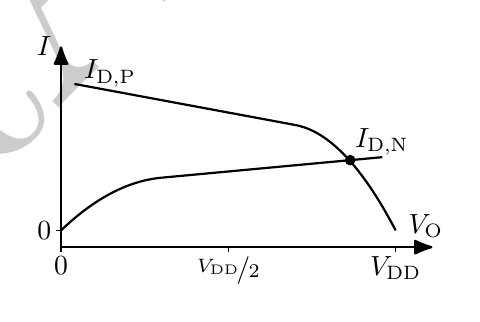
\begin{tikzpicture}[scale=0.85]
      \node[anchor=north] at (0,0) {0};
      \draw[thin] (0,0) -- (0,-0.075);
      \node[anchor=east] at (0,0.25) {0};
      \draw[thin] (0,0.25) -- (-0.075,0.25);

      \node[anchor=north] at (2.5,0) {$\nicefrac{V_{\mathrm{DD}}}{2}$};
      \draw[thin] (2.5,0) -- (2.5,-0.075);
      \node[anchor=north] at (5.0,0) {$V_{\mathrm{DD}}$};
      \draw[thin] (5.0,0) -- (5.0,-0.075);

      \draw[{Latex[round,scale=1.2]}-{Latex[round,scale=1.2]},thick] 
        (0,3) -- (0,0) -- (5.55,0);

      \node[anchor=south] at (5.45,0) {$V_{\mathrm{O}}$};
      \node[anchor=east] at (0,3) {$I$};

      \draw[thick] plot[smooth,domain=0:1.5] (\x, {0.25-0.288016529*\x^2+0.957024794*\x});
      \draw[thick] plot[smooth,domain=1.5:4.8] (\x, {0.092975206*(\x-1.5)+1.0375)});

      \draw[thick] plot[smooth,domain=3.5:5] (\x, {0.25-0.576033058*(5-\x)^2+1.914049588*(5-\x)});
      \draw[thick] plot[smooth,domain=0.2:3.5] (\x, {0.185950413*((5-\x)-1.5)+1.825)});

      \node[anchor=south west] at (0.2,2.25) {$I_{\mathrm{D,P}}$};
      \node[anchor=south west] at (4.25,1.23) {$I_{\mathrm{D,N}}$};

      \filldraw (4.32,1.3) circle (2pt);
    \end{tikzpicture}
    \caption{Slow NMOS}
    \label{fig:currplot:slownmos} 
  \end{subfigure}
  \hfill
  \begin{subfigure}[b]{0.31\textwidth}
    \centering
    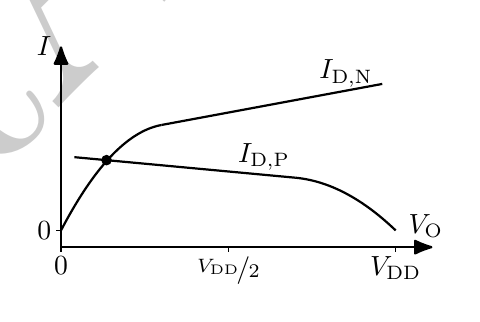
\begin{tikzpicture}[scale=0.85]
      \node[anchor=north] at (0,0) {0};
      \draw[thin] (0,0) -- (0,-0.075);
      \node[anchor=east] at (0,0.25) {0};
      \draw[thin] (0,0.25) -- (-0.075,0.25);

      \node[anchor=north] at (2.5,0) {$\nicefrac{V_{\mathrm{DD}}}{2}$};
      \draw[thin] (2.5,0) -- (2.5,-0.075);
      \node[anchor=north] at (5.0,0) {$V_{\mathrm{DD}}$};
      \draw[thin] (5.0,0) -- (5.0,-0.075);

      \draw[{Latex[round,scale=1.2]}-{Latex[round,scale=1.2]},thick] 
        (0,3) -- (0,0) -- (5.55,0);

      \node[anchor=south] at (5.45,0) {$V_{\mathrm{O}}$};
      \node[anchor=east] at (0,3) {$I$};

      \draw[thick] plot[smooth,domain=0:1.5] (\x, {0.25-0.576033058*\x^2+1.914049588*\x});
      \draw[thick] plot[smooth,domain=1.5:4.8] (\x, {0.185950413*(\x-1.5)+1.825)});

      \draw[thick] plot[smooth,domain=3.5:5] (\x, {0.25-0.288016529*(5-\x)^2+0.957024794*(5-\x)});
      \draw[thick] plot[smooth,domain=0.2:3.5] (\x, {0.092975206*((5-\x)-1.5)+1.0375)});

      \node[anchor=south west] at (2.5,1) {$I_{\mathrm{D,P}}$};
      \node[anchor=south east] at (4.8,2.25) {$I_{\mathrm{D,N}}$};

      \filldraw (0.68,1.3) circle (2pt);
    \end{tikzpicture}
    \caption{Slow PMOS}
    \label{fig:currplot:slowpmos}
  \end{subfigure}
  \caption{Plot}
  \label{fig:currplot}
\end{figure}

\printbibliography

\end{document}